% !TEX root = ../thesis.tex
% =============================================================================
% Chapter 4: Methodology
% =============================================================================

\chapter{Methodology}
\label{ch:methodology}

This chapter describes the experimental pipeline used to answer the research questions posed in \cref{ch:introduction}. The pipeline runs in four stages. Stage~1 screens ten LLMs and identifies the strongest model for algorithm generation. Stage~2 analyses the resulting trajectories and selects an informative subset of behavioural features. Stage~3 tests three framings of those features as feedback to the LLM. Stage~4 brings the chosen model, features, and framing together in a full-benchmark head-to-head comparison against vanilla and SAGE feedback baselines. We first describe the LLaMEA framework and benchmark configuration that underpin all four stages.

% ---------------------------------------------------------------------------
\section{LLaMEA Framework}
\label{sec:meth-llamea}

Vanilla LLaMEA operates a $(1 + 1)$-ES loop, summarised in \cref{alg:llamea}. Every run starts from a shared initial algorithm, \texttt{RandomSearch}, which performs uniform random sampling across the search space and returns the best sample found. Pre-seeding the population this way ensures that all models and conditions begin from identical starting conditions, so observed differences are attributable to the LLM and the feedback rather than to initialisation luck.

\begin{algorithm}[t]
\caption{$(1+1)$-LLaMEA evolutionary loop, adapted from \cite{vanStein2024LLaMEA}.}
\label{alg:llamea}
\SetKwInOut{Input}{Input}
\SetKwInOut{Output}{Output}
\Input{Task prompt $S$, feedback prompt template $F_0$, budget $T$}
\Output{Best algorithm $a_b$ and its quality $y_b$}
$a_0 \gets \text{LLM}(S)$\;
$(y_0, \sigma_0, e_0) \gets f(a_0)$\;
$a_b \gets a_0;\; y_b \gets y_0$\;
\For{$t \gets 1$ \KwTo $T$}{
  $F \gets (S,\; \{(\text{name}(a_i), y_i)\}_{i=0}^{t},\; (a_b, y_b, \sigma_b),\; F_0)$\;
  $a_{t} \gets \text{LLM}(F)$\;
  $(y_{t}, \sigma_{t}, e_{t}) \gets f(a_{t})$\;
  \If{$e_{t} \neq \varnothing$}{$y_{t} \gets 0$}
  \If{$y_{t} \geq y_b$}{$a_b \gets a_{t};\; y_b \gets y_{t};\; \sigma_b \gets \sigma_{t}$}
}
\Return{$a_b, y_b$}
\end{algorithm}

\begin{figure*}[!t]
  \centering
  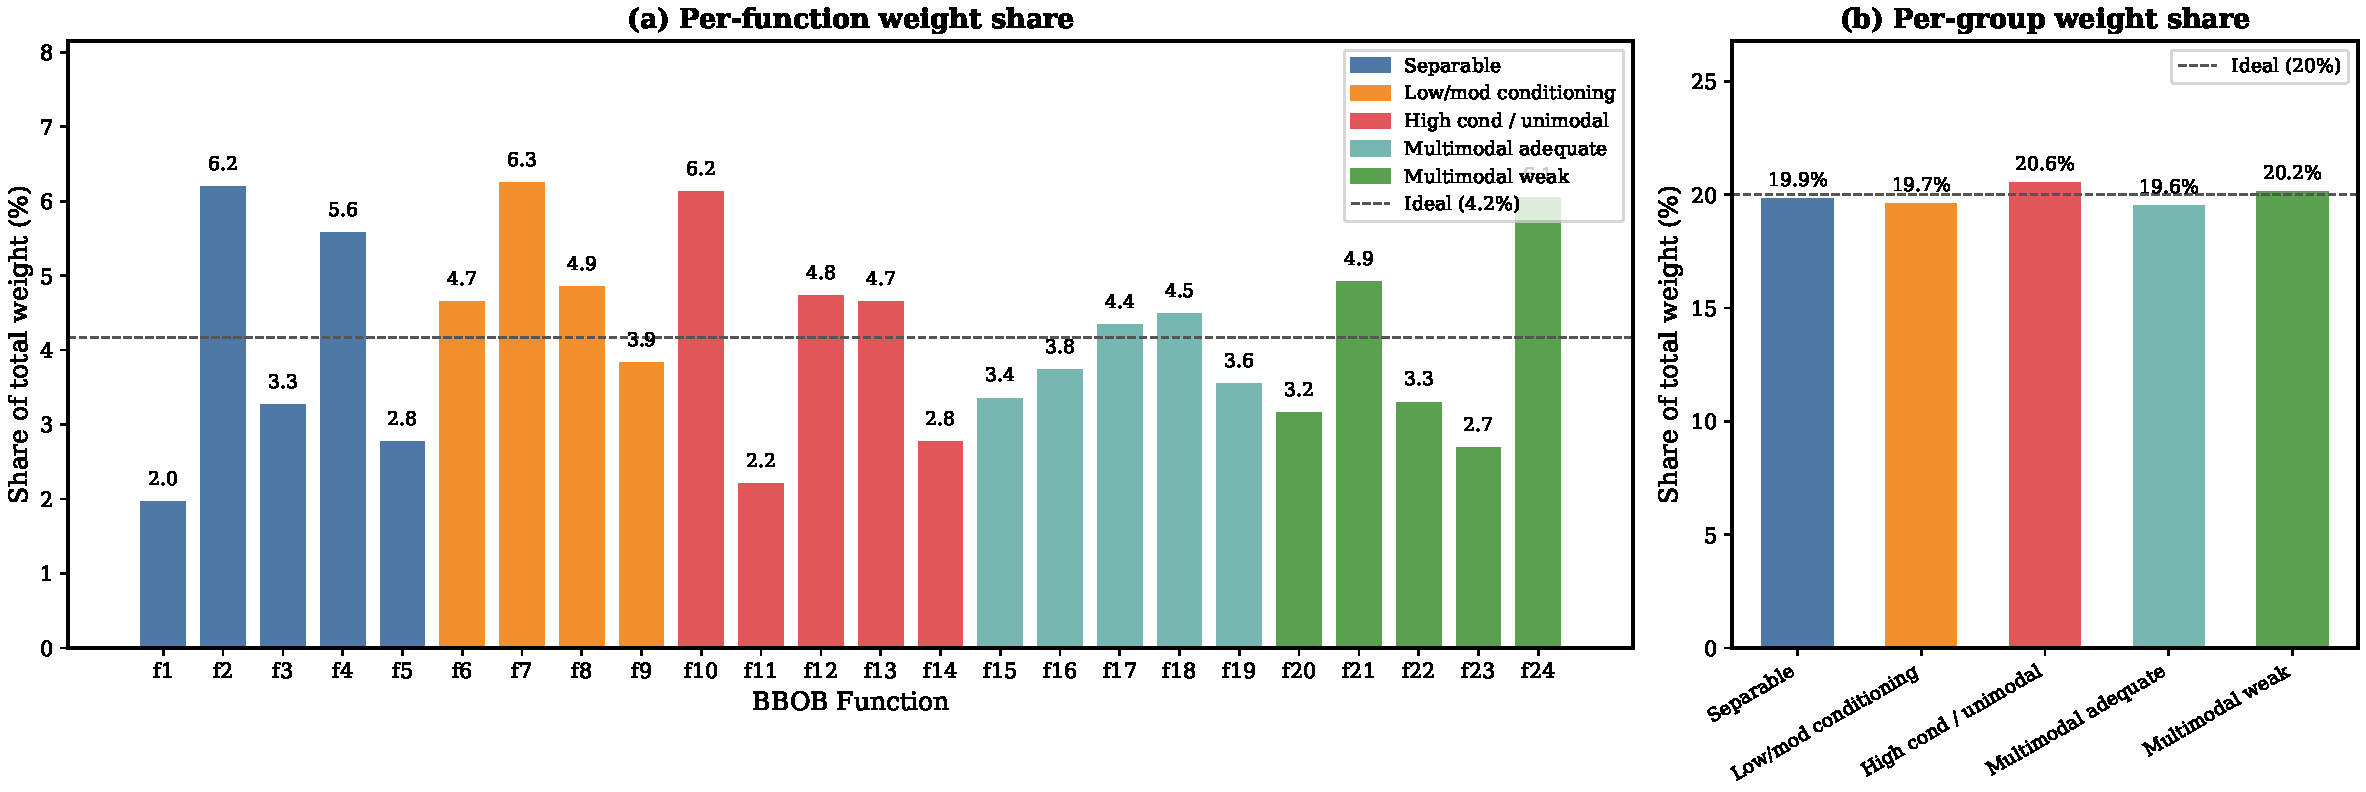
\includegraphics[width=\textwidth]{figures/fig_mabbob_instances.pdf}
  \caption{BBOB function weight distribution of the selected 10 MA-BBOB functions, coloured by BBOB function group. All 24 BBOB functions are covered with near-uniform balance.}
  \label{fig:mabbob-instances}
\end{figure*}

\begin{table*}[!t]
\centering
\caption{BBOB function weights for the 10 selected MA-BBOB functions. Only non-zero contributions are shown (as percentage of total weight). BBOB functions are grouped into separable (f1--f5), low/moderate conditioning (f6--f9), high conditioning/unimodal (f10--f14), multimodal adequate (f15--f19), multimodal weak (f20--f24).}
\label{tab:instance-weights}
\footnotesize
\begin{tabular}{@{}r|ccccc|cccc|ccccc|ccccc|ccccc@{}}
\toprule
& \multicolumn{5}{c|}{\textbf{Sep.}} & \multicolumn{4}{c|}{\textbf{Low/mod}} & \multicolumn{5}{c|}{\textbf{High/uni}} & \multicolumn{5}{c|}{\textbf{MM adeq.}} & \multicolumn{5}{c}{\textbf{MM weak}} \\
\textbf{Func.} & \footnotesize 1 & \footnotesize 2 & \footnotesize 3 & \footnotesize 4 & \footnotesize 5
& \footnotesize 6 & \footnotesize 7 & \footnotesize 8 & \footnotesize 9
& \footnotesize 10 & \footnotesize 11 & \footnotesize 12 & \footnotesize 13 & \footnotesize 14
& \footnotesize 15 & \footnotesize 16 & \footnotesize 17 & \footnotesize 18 & \footnotesize 19
& \footnotesize 20 & \footnotesize 21 & \footnotesize 22 & \footnotesize 23 & \footnotesize 24 \\
\midrule
191 & & & & & & 28 & & & & & & & & & & & & & 25 & 21 & 1 & & 25 & \\
277 & 15 & & 14 & & & & 10 & & & 13 & & & 13 & 6 & & & & 20 & & & & 6 & & 4 \\
300 & & & 19 & & & & 20 & & & & & 18 & & & & & & 12 & & & 29 & & 2 & \\
412 & & 10 & & & 12 & & & 13 & & 14 & & & & & & & 11 & & 11 & & & & & 29 \\
455 & & 13 & & & & & & 17 & & 14 & 14 & & & & & & & 14 & & & & & & 28 \\
635 & & & & 23 & 4 & & 13 & & & & & 9 & & 16 & & 23 & & & & & & 14 & & \\
648 & 5 & & & 9 & & & 20 & & 18 & & & & 18 & & 17 & & & & & 11 & 2 & & & \\
744 & & 17 & & & & 19 & & & & 10 & & & & 7 & 17 & 15 & 15 & & & & & & & \\
760 & & 1 & & 9 & 12 & & & 4 & 20 & & 7 & & 15 & & & & & & & & 17 & 14 & & \\
843 & & 21 & & 14 & & & & 14 & & 10 & 2 & 20 & & & & & 18 & & & & & & & \\
\bottomrule
\end{tabular}
\\[0.3em]
{\scriptsize Values are percentages of total weight. Empty cells indicate zero weight.}
\end{table*}

At each generation the LLM receives a prompt assembled from a role description, a task specification, an example algorithm, a feedback string reporting that algorithm's performance, an optional mutation prompt, and an output-format constraint. The role, task, and output-format portions are taken verbatim from LLaMEA~\cite{vanStein2024LLaMEA}. The full prompt template is shown below.

\begin{lstlisting}[numbers=none,breakautoindent=false,breakindent=0pt,xleftmargin=0pt,basicstyle=\ttfamily\scriptsize]
You are a highly skilled computer scientist in the field of natural computing. Your task is to design novel metaheuristic algorithms to solve black box optimization problems.

The optimization algorithm should handle a wide range of tasks, which is evaluated on the BBOB test suite of 24 noiseless functions. Your task is to write the optimization algorithm in Python code to minimize the function value. The code should contain an `__init__(self, budget, dim)` function and the function `def __call__(self, func)`, which should optimize the black box function `func` using `self.budget` function evaluations.

The func() can only be called as many times as the budget allows, not more. Each of the optimization functions has a search space between -5.0 (lower bound) and 5.0 (upper bound). The dimensionality can be varied.

Give an excellent and novel heuristic algorithm to solve this task.

An example of such code is as follows:
<example algorithm>

Feedback:

The algorithm <algorithm name> got an average Area over the convergence curve (AOCC, 1.0 is the best) score of <score> with standard deviation <std>.

<mutation prompt>

Provide the Python code and a one-line description with the main idea (without enters). Give the response in the format:
# Description: <short-description>
# Code:
```python
<code>
```
\end{lstlisting}

On the first generation the example is \texttt{RandomSearch} (reproduced in \cref{app:randomsearch}) and no mutation prompt is added. From the second generation onwards, the previous best algorithm replaces \texttt{RandomSearch} as the example, and the mutation prompt is drawn from the dual-prompt configuration identified as effective by van Stein et al.~\cite{vanStein2025Behaviour}. With 90\% probability the LLM receives a \emph{refine} prompt (``\textit{Refine and simplify the selected algorithm to improve it}''), and with 10\% probability an \emph{explore} prompt (``\textit{Generate a new algorithm that is different from those tried before}''). This split balances exploitation of promising algorithm structures with exploration of novel designs. The 90/10 ratio is our own choice and to our knowledge no systematic study of its optimality exists.

The offspring then competes against its parent under elitist $(1+1)$ selection. It replaces the parent only if it achieves equal or better fitness, and the surviving algorithm becomes the parent for the next generation. Recent work has explored larger population sizes. Van Stein et al.~\cite{vanStein2025Behaviour} compare six LLaMEA configurations including population-based variants with $\mu/\lambda = 4/12$, and the SAGE experiments~\cite{vanStein2026LLaMEASAGE} use $4$ parents and $16$ offspring. Among the six configurations in the Behaviour Space study~\cite{vanStein2025Behaviour}, the elitist $(1+1)$ variant (LLaMEA-4) outperformed the population-based alternatives, and we retain it for that reason.

After each evaluation, the LLM receives a feedback string reporting the algorithm's performance. Standard (vanilla) feedback reports only the AOCC score and its standard deviation across evaluation runs. Our experiments augment this string with additional behavioural feature information detailed in in \cref{sec:meth-feedback-screening}.

% ---------------------------------------------------------------------------
\section{Benchmark Configuration}
\label{sec:meth-benchmark}

Candidate algorithms are evaluated on MA-BBOB~\cite{vermetten2023mabbob}. Each MA-BBOB function is parameterised by a weight vector over the 24 BBOB functions. All functions used in this thesis are 5-dimensional with search bounds $[-5, 5]^5$.

This thesis uses two function sets drawn from the same 1{,}000-function MA-BBOB pool. The first three stages use a ten-function set, sized to discriminate between models, features, and feedback formats while keeping screening compute tractable across the many models, conditions, and seed replicates that those stages require. Stage~4 uses an extended twenty-function set, disjoint from the screening set, both to give the head-to-head comparison tighter AOCC variance bands and to test that the conclusions of Stages~1--3 generalise to functions the pipeline was not implicitly tuned on.

Both function sets are selected by the greedy forward procedure in \cref{alg:instance-selection}. At each step every remaining function is scored as a potential addition to the current set, with the score favouring candidates that cover BBOB functions not yet represented, that bring the five group shares closer to the ideal 20\% each, and that distribute weight evenly across BBOB functions. Missing BBOB function coverage dominates the score, ensuring all 24 BBOB functions are included before the procedure optimises for balance among individual BBOB function representation. For the ten-function screening set the resulting selection covers all 24 BBOB functions with group shares within $\pm$0.6\% of the ideal 20\% (\cref{fig:mabbob-instances}). \cref{tab:instance-weights} shows the per-function weight breakdown, where each MA-BBOB function blends between 5 and 9 BBOB functions.

\begin{algorithm}[t]
\caption{Greedy MA-BBOB function selection. At each step the candidate whose addition most reduces missing BBOB function count, group imbalance, and per-BBOB-function weight variability is selected.}
\label{alg:instance-selection}
\SetKwInOut{Input}{Input}
\SetKwInOut{Output}{Output}
\Input{$\mathbf{W} \in \mathbb{R}^{1000 \times 24}$ (weight matrix), $k = 10$}
\Output{Selected function set $S$}
$S \gets \varnothing$\;
\For{$i \gets 1$ \KwTo $k$}{
  \ForEach{$c \notin S$}{
    $\mathbf{w} \gets$ column sums of $\mathbf{W}[S \cup \{c\}]$\;
    $m \gets |\{j : w_j = 0\}|$\;
    $\sigma_g \gets \operatorname{std}(\{w_g / \sum w : g \in \text{groups}\})$\;
    $\mathrm{CV} \gets \operatorname{std}(\mathbf{w}_{>0}) / \operatorname{mean}(\mathbf{w}_{>0})$\;
    $\operatorname{score}(c) \gets -100\,m - 10\,\sigma_g - \mathrm{CV}$\;
  }
  $c^* \gets \arg\max_c \;\operatorname{score}(c)$\;
  $S \gets S \cup \{c^*\}$\;
}
\Return{$S$}
\end{algorithm}

The twenty-function Stage~4 set is produced by the same procedure with the ten-function screening set excluded from the candidate pool, ensuring disjointness. The resulting subset covers all 24 BBOB functions with a coefficient of variation of $0.080$ across BBOB function weight totals, and gives the five BBOB function groups shares within $\pm$1.3\% of the ideal 20\%. The BBOB function weight distribution and per-function breakdown are reported in \cref{app:instance-selection-stage4}.

This selection procedure was used to mitigate design bias inherited from the underlying BBOB function set. MA-BBOB is itself a technique for reducing such bias by allowing arbitrary affine combinations of the 24 base functions, but because our function sets are sampled from a finite MA-BBOB pool, residual structure from BBOB persists. The base functions share landscape characteristics within their group as exposed by exploratory landscape analysis~\cite{long2023bbobinstance}, and the five groups are unevenly populated (4 functions in low/moderate conditioning, 5 in each of the others). Selecting for uniform BBOB-function coverage and balanced group shares at the contribution-weight level minimises the influence of any single function or group on aggregated performance, though some residual bias from the fixed BBOB pool is unavoidable.

Each candidate algorithm is evaluated on every function in the active set over 5 configuration instances. For Stages~1--3 this yields 50 independent runs per candidate (10 functions $\times$ 5 instances) and for Stage~4 it yields 100 (20 functions $\times$ 5 instances). The evaluation budget per run is $T = 2{,}000 \times d = 10{,}000$ function evaluations (FEs), following the BBOB convention~\cite{hansen2021coco}.

Algorithm quality is measured by the Area Over the Convergence Curve (AOCC). For a single run of algorithm $a$ on function $f$ and instance $s$, with evaluation budget $T$, the normalised per-run area is:
\begin{equation}
\label{eq:per-run-area}
A(\mathbf{y}_{a,f,s}) = \frac{1}{T} \sum_{t=1}^{T} \left(1 - \frac{\min(\max(y_t, lb), ub) - lb}{ub - lb}\right)
\end{equation}
where $\mathbf{y}_{a,f,s} = (y_1, \ldots, y_T)$ is the sequence of log-scaled best-so-far fitness values, and $ub = 10^{2}$, $lb = 10^{-8}$ are the clipping bounds. The AOCC for a candidate algorithm is the mean of $A$ over all functions $f$ and instances $s$:
\begin{equation}
\label{eq:aocc}
\text{AOCC}(a) = \frac{1}{N} \sum_{f=1}^{F} \sum_{s=1}^{S} A(\mathbf{y}_{a,f,s})
\end{equation}
In Stages~1--3 we have $F = 10$ and $S = 5$, giving $N = 50$ independent runs per candidate. Stage~4 uses $F = 20$, raising $N$ to 100. This single scalar is reported to the LLM as feedback.

For every successful candidate evaluation, the full trajectory ($T = 10{,}000$ evaluations of decision variables and fitness values) is logged via IOHexperimenter, and all 32 behavioural features described in \cref{ch:features} are computed post-hoc. Features are averaged across the 50 runs per candidate to produce a single feature vector per algorithm. This dataset, comprising feature vectors for every valid candidate across all models and seeds, forms the basis for the Stage~2 feature analysis.

% ---------------------------------------------------------------------------
\section{LLM Screening}
\label{sec:meth-screening}

Stage~1 screens LLMs for their ability to reliably generate high-quality metaheuristics for continuous black-box optimisation. Small language models vary substantially in their ability to generate valid optimisation code, and inference cost matters when each evolutionary run requires hundreds of LLM calls. The screening identifies the model that is later carried forward into Stages~3 and~4, and supplies the dataset of trajectories on which Stage~2 is built.

Ten models are evaluated, spanning locally served open-weight models and cloud API models. \cref{tab:models} lists all models with their parameter counts and providers. Each model runs the LLaMEA loop for 100 candidates across 5 independent seeds, all using vanilla AOCC-only feedback, for a total of $10 \text{ models} \times 5 \text{ seeds} \times 100 \text{ candidates} = 5{,}000$ LLaMEA iterations. All 32 behavioural features are computed for every successful candidate, producing a dataset of several thousand algorithm--feature observations.

\begin{table}[t]
\centering
\caption{LLMs evaluated in Stage~1. Local models are served via Ollama~\cite{ollama} or vLLM~\cite{kwon2023vllm}. API models use Google's Gemini API. Parameter counts reflect total (not active) parameters.}
\label{tab:models}
\footnotesize
\begin{tabular}{@{}llrl@{}}
\toprule
\textbf{Model} & \textbf{Provider} & \textbf{Params} & \textbf{Backend} \\
\midrule
Qwen3.5 4B   & Qwen/Alibaba~\cite{qwen3}          & 4B  & Ollama \\
Qwen3.5 9B   & Qwen/Alibaba~\cite{qwen3}          & 9B  & vLLM \\
Qwen3.5 27B  & Qwen/Alibaba~\cite{qwen3}          & 27B & Ollama \\
RNJ-1 8B     & Essential AI~\cite{rnj1}            & 8B  & Ollama \\
Devstral Small~2 & Mistral AI~\cite{devstral2}     & 24B & Ollama \\
OLMo~3 7B    & Allen AI~\cite{olmo3}               & 7B  & Ollama \\
OLMo~3 32B Think & Allen AI~\cite{olmo3}           & 32B & Ollama \\
Granite~4 Micro  & IBM~\cite{granite4}             & 3B  & vLLM \\
\midrule
Gemini~3 Pro     & Google~\cite{gemini3pro}      & --- & API \\
Gemini~3 Flash   & Google~\cite{gemini3flash}      & --- & API \\
\bottomrule
\end{tabular}
\end{table}

Models are compared on three factors. The failure rate is the fraction of candidates that fail to produce valid fitness, due to syntax errors, interface mismatches, or runtime exceptions. The best AOCC is the highest AOCC achieved across all 5 seeds, measuring peak algorithm quality. The inference efficiency is the rate of tokens generated per second, which determines wall-clock time per evolutionary run. The model that performs best across these factors is carried forward into later stages.

% ---------------------------------------------------------------------------
\section{Feature Analysis and Selection}
\label{sec:meth-feature-selection}

Stage~2 analyses the Stage~1 dataset of behavioural feature vectors for all valid candidates across 10 models and 5 seeds to determine which of the 32 features in \cref{ch:features} are most predictive of algorithm quality, and to select a tractable subset for the feedback experiments. The target subset size is fixed at ten features. The cap is set by the available compute budget and API costs rather than statistical considerations. Stage~3 evaluates each retained feature in three framings across 5 seeds of 100 candidates with the model identified in Stage~1, and the per-feature cost of running these evaluations makes a larger subset infeasible. Selecting on predictive power keeps the ten most informative features in the loop, while pruning redundancy ensures they capture distinct aspects of behaviour rather than re-stating the same signal.

Three complementary approaches are applied to rank the 32 features, each capturing a different aspect of feature quality. Spearman rank correlation~\cite{spearman1904proof} captures monotonic associations between each feature and AOCC across all valid candidates, regardless of functional form. Random Forest permutation importance~\cite{breiman2001randomforests} captures non-linear and interaction effects. A regression model is trained to predict AOCC from all 32 features, and each feature's importance is measured by the decrease in out-of-bag $R^2$ when its values are permuted. Kolmogorov--Smirnov distributional effect size~\cite{kolmogorov1933} captures distributional separation between high- and low-quality algorithms. It computes the KS statistic between feature distributions of the top-25\% and bottom-25\% candidates by AOCC, after winsorising each feature at the 1st and 99th percentiles to limit the influence of outliers.

Each method produces a ranked list of 32 features. The three rankings are aggregated via Borda count~\cite{black1958theory}. Each feature receives $32 - r_i$ points from each method (where $r_i$ is its rank in method $i$). Summed scores determine the consensus ranking, with lower values indicating a more informative feature.

The consensus list is then de-duplicated by greedy redundancy pruning. Features are processed in Borda-rank order. If a candidate feature has Spearman $|\rho| > \tau$ with any already-selected feature, it is discarded as redundant. To determine $\tau$ we sweep across the range $[0.5, 1.0]$ in steps of $0.05$ and record, at each value, the surviving subset and its mean Borda rank, then pick the value that produces the largest single-step improvement in mean Borda rank. This corresponds to the elbow in the quality-vs-threshold curve, beyond which further tightening prunes already-distinct features without comparable gain. The top ten survivors of pruning at this threshold form the final feature subset taken into Stage~3.

% ---------------------------------------------------------------------------
\section{Feedback Format Screening}
\label{sec:meth-feedback-screening}

Stage~3 tests whether the framing of behavioural feedback affects the performance of LLM-generated algorithms. Each feature selected in Stage~2 is embedded into the feedback string under three contrasting framings (neutral, directional, comparative), with one feature added at a time so that effects can be attributed to the framing rather than to the joint presence of multiple features. The comparative format is excluded for \texttt{longest\_no\_improvement\_streak} because that feature has a U-shaped relationship with AOCC for which a single reference target would be misleading, leaving 29 active conditions.

The neutral format reports the feature value and its definition, without any indication of whether high or low values are desirable,

\begin{quote}
\small\itshape
The algorithm X got an average AOCC score of 0.7234 with standard deviation 0.0891. It achieved a \texttt{step\_size\_autocorrelation} of 0.8421 with standard deviation 0.0532, which measures whether large steps tend to follow large steps, capturing momentum in the search.
\end{quote}

The directional format extends the neutral format with a sentence indicating which direction is associated with better performance. The direction is derived from the prior Spearman correlation analysis,

\begin{quote}
\small\itshape
\ldots capturing momentum in the search. Higher values are associated with better performance, indicating consistent, smooth step-size adaptation rather than erratic jumps.
\end{quote}

The comparative format replaces the directional guidance with a distance-aware comparison against a concrete reference value. The reference is the median feature value of top-10\% algorithms by AOCC from the LLM screening stage. The normalised distance from this reference is $d = (v_{\text{ref}} - v) / (v_{\text{ref}} - v_{\text{bot25}})$, where $v$ is the candidate's feature value, $v_{\text{ref}}$ is the top-10\% median, and $v_{\text{bot25}}$ is the bottom-25\% median. This denominator provides a meaningful scale representing the range between good and bad algorithms for each feature. The numeric reference value is reported in every tier so that the LLM has a concrete target rather than only a qualitative direction. The wording of the comparison itself adapts across four tiers, strengthening progressively as $d$ grows:

\begin{enumerate}
  \item \textbf{Already meets reference} ($d \leq 0$): ``\textit{This already meets or exceeds the top-performing reference of 0.9070. Maintain this.}''
  \item \textbf{Close to reference} ($0 < d \leq 0.15$): ``\textit{This is close to the top-performing reference of 0.9070. A small increase could help.}''
  \item \textbf{Moderate gap} ($0.15 < d \leq 0.50$): ``\textit{This is moderately below the top-performing reference of 0.9070. Consider increasing this value.}''
  \item \textbf{Far from reference} ($d > 0.50$): ``\textit{This is far from the reference of 0.9070. Increasing this value is a priority.}''
\end{enumerate}

Each condition runs for 100 candidates across 5 independent seeds, for a total of $29 \text{ conditions} \times 5 \text{ seeds} \times 100 \text{ candidates} = 14{,}500$ LLaMEA iterations, and the vanilla AOCC-only results from Stage~1 serve as the baseline for measuring performance improvements.

% ---------------------------------------------------------------------------
\section{Full-Benchmark Comparison}
\label{sec:meth-stage4}

\begin{figure*}[!t]
  \centering
  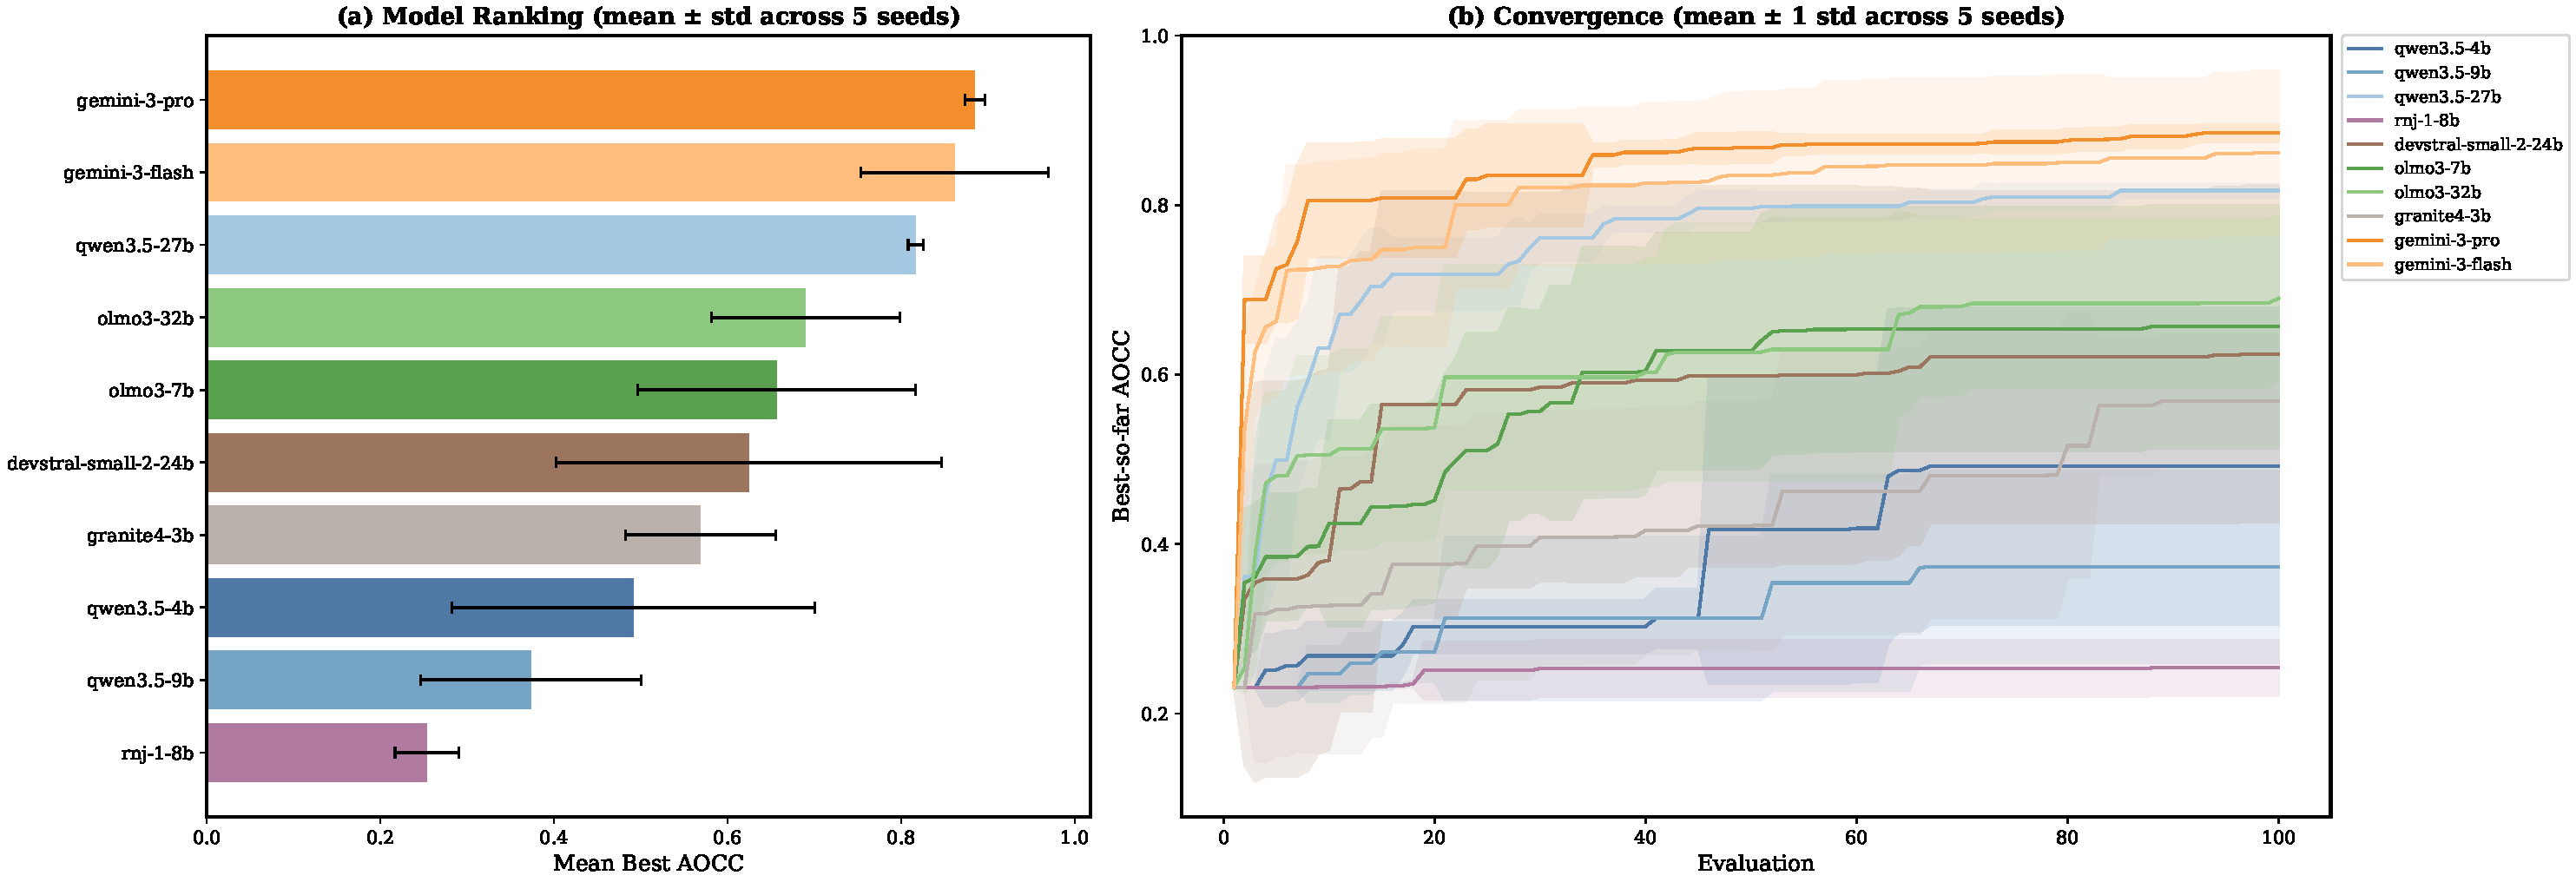
\includegraphics[width=\textwidth]{figures/fig_model_screening.pdf}
  \caption{LLM screening results. (a)~Mean best AOCC by model ($\pm$ std across 5 seeds). (b)~Best-so-far AOCC over 100 evaluations, averaged across 5 seeds. Shaded regions show $\pm$1 std.}
  \label{fig:model-screening}
\end{figure*}

\begin{table}[t]
\centering
\caption{Stage~1 model ranking (100 candidates $\times$ 5 seeds, vanilla feedback). Fail\% and AOCC averaged across seeds ($\pm$ std).}
\label{tab:model-ranking}
\footnotesize
\begin{tabular}{@{}rlrrr@{}}
\toprule
\textbf{\#} & \textbf{Model} & \textbf{Fail\%} & \textbf{AOCC} & \textbf{h/run} \\
\midrule
1  & Gem.~3 Pro    & 10.2  & .885$\pm$.011 & 5.1 \\
2  & Gem.~3 Flash  & \textbf{2.0} & .862$\pm$.108 & 3.9 \\
3  & Qwen3.5 27B   & 41.0  & .817$\pm$.009 & 38.9 \\
4  & OLMo~3 32B    & 13.2  & .690$\pm$.109 & 39.3 \\
5  & OLMo~3 7B     & 27.6  & .657$\pm$.160 & 18.4 \\
6  & Devstral~2    & 32.6  & .625$\pm$.222 & 5.0 \\
7  & Granite~4 3B  & 53.8  & .569$\pm$.087 & \textbf{0.6} \\
8  & Qwen3.5 4B    & 76.2  & .492$\pm$.209 & 7.9 \\
9  & Qwen3.5 9B    & 91.6  & .373$\pm$.127 & 3.0 \\
10 & RNJ-1 8B      & 34.6  & .254$\pm$.037 & 14.5 \\
\bottomrule
\end{tabular}
\end{table}

Stage~4 is a head-to-head comparison of four feedback conditions, run on the twenty-function MA-BBOB set with longer evolutionary runs and more independent seeds than the screening stages so condition differences can be detected at the resolution required to draw substantive conclusions.

The vanilla condition uses AOCC-only feedback, identical to the baseline used in Stage~1, repeated here on the new function set as the reference point against which all other conditions are measured. The neutral condition extends AOCC with trajectory-derived behavioural features, isolating the contribution of distal (behavioural) feedback. The sage condition pairs AOCC with structural code-level guidance from LLaMEA-SAGE~\cite{vanStein2026LLaMEASAGE}, used unmodified, isolating the contribution of proximal (structural) feedback. The combined condition appends both behavioural and structural feedback in the same prompt, testing whether the two channels are complementary or redundant.

The behavioural feedback uses the five features ranked highest by mean best AOCC across the Stage~3 neutral conditions. These features are \texttt{intensification\_ratio}, \texttt{dimension\_convergence\_heterogeneity}, \texttt{fitness\_plateau\_fraction}, \texttt{avg\_improvement}, and \texttt{improvement\_spatial\_correlation}. All five are appended to the AOCC feedback string in the neutral framing. The five-feature cap keeps the prompt compact while still spanning the four functional categories of \cref{ch:features} (intensification, convergence, stagnation, and exploration).

Benchmark parameters from \cref{sec:meth-benchmark} are inherited unchanged, with the Stage~4 function set detailed in \cref{app:instance-selection-stage4}. Each condition runs for 500 candidates per seed, five times the screening budget, giving feedback signals that act gradually a fair chance to express their effect. Ten independent seeds per condition (double the previous stages) tighten the variance bands when comparing condition means and make condition-vs-condition differences detectable at smaller effect sizes. The total compute is $4 \text{ conditions} \times 10 \text{ seeds} \times 500 \text{ candidates} = 20{,}000$ candidate algorithms, each evaluated over $20 \text{ functions} \times 5 \text{ instances} = 100$ MA-BBOB runs hence totalling 2,000,000 MA-BBOB function evaluations.

Finally, to assess how the strongest generated algorithms generalise beyond the twenty-function set and the 5-dimensional regime in which they were developed, the best-found algorithm from each of the conditions is re-evaluated on the full $1{,}000$-instance MA-BBOB pool. A generic CMA-ES~\cite{hansen2001cmaes} and \texttt{NeighborhoodAdaptiveDE} (NADE)~\cite{vanStein2025NeighborhoodDE}, the winner of the 2025 MA-BBOB competition, are used as basline performance references. Each of the six algorithms runs on all $1{,}000$ MA-BBOB functions across 5 instance seeds and three dimensionalities $d \in \{5, 10, 20\}$, under a $2{,}000d$ FE budget per run, totalling approximately $2.1 \times 10^9$ function evaluations.

% ---------------------------------------------------------------------------
\section{Infrastructure}
\label{sec:meth-infrastructure}

All experiments are executed on the LIACS SLURM cluster node \textbf{saronite}, equipped with 4$\times$ NVIDIA L40S GPUs (48\,GB each), 2$\times$ 32-core Intel Xeon Gold 6438M CPUs, and 512\,GB RAM. Most local models are served via Ollama~\cite{ollama}, which processes requests sequentially in a queue. For Qwen3.5~9B and Granite~4~Micro, we use vLLM~\cite{kwon2023vllm}, which supports continuous batching and manages KV caches efficiently via PagedAttention~\cite{kwon2023vllm}. This allows multiple seeds to issue concurrent inference requests rather than waiting in a serial queue, reducing wall-clock time per evolutionary run. Gemini~3 models~\cite{gemini3pro, gemini3flash} are accessed through Google's Gemini API. All code, configuration, and analysis notebooks are available in the thesis repository.\footnote{\url{https://github.com/maxharell/thesis}} The BLADE~\cite{vanStein2025BLADE} and LLaMEA~\cite{vanStein2024LLaMEA} repositories are included as Git submodules, with minor modifications to support custom feedback strings and extended behavioural metric logging.
